\documentclass{article}

\usepackage[frenchb]{babel}
\usepackage[utf8x]{inputenc}
\usepackage[pdftex]{color,graphicx}
\usepackage{amssymb, amsmath}
\usepackage{verbatim}

\begin{document}

\title{
  École Polytechnique de Montréal \\
  Physique pour les applications multimédia \\
  PHS4700 \\
  Projet
}

\author{
  Emmanuel Boudreault (1336476) \\
  Catherine Sanschagrin (1232199)
}

\date{9 decembre 2011}

\maketitle

\newpage

\section*{Description du problème}

Il nous est demandé de créer une simulation d'une partie de croquet de
jardin entre deux joueurs. Le jeux de croquet comporte six anneaux que
l'on doit parcourir dans un ordre précis. Le terrain mesures 14 m par
17.5 m. Il est délimité par un mur d'une hauteur de 10 cm avec des
coins qui ne sont pas carrée. Au centre du terrain, il y a un poteau
avec un diamètre de 2 cm et une hauteur de 50 cm.

Les murs diagonaux ont l'air de ceci:

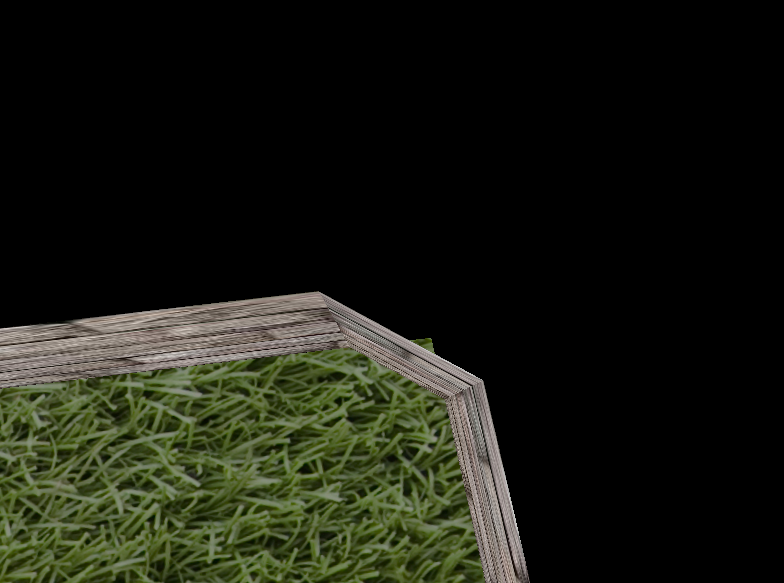
\includegraphics[width=4in]{wall.png}

Les six cerceaux sont bâtis avec des tiges qui ont 1.5 cm de diamètre
et une hauteur de 30 cm. L'espace dans lequel les balles peuvent
passer est large de 10 cm. Les cerceaux sont placés comme le suit:

\begin{tabular}{| c | c | c |}
\hline
Cerceau & x (m) & y (m) \\
\hline
1 & -3.5 & -5.25 \\
2 & -3.5 & 5.25 \\
3 & 3.5 & 5.25 \\
4 & 3.5 & -5.25 \\
5 & 0.0 & -3.5 \\
6 & 0.0 & 3.5 \\
\hline
\end{tabular}

Nous pouvons voir ce que cela donne plus bas:

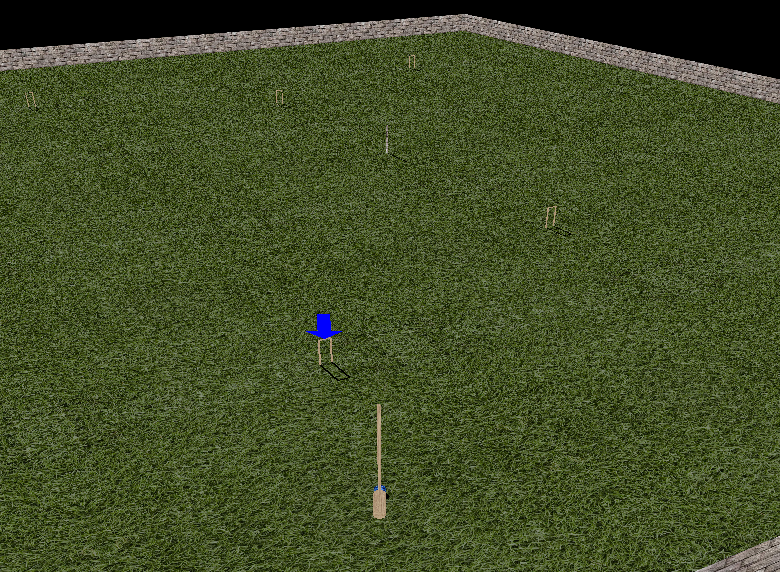
\includegraphics[width=4in]{field.png}

Il est à noter que l'énoncer avait les mêmes coordonnées pour les
cerceaux 5 et 6. Nous avec donc inversé la composante en y pour le
sixième cerceau.

Les boules on un diamètre de 7.6 cm avec une masse volumique de 1.109
$g / cm^3$ ce qui donne une masse d'environ 0.254 kg.

Les maillets ont une masse de 1.25 kg avec la tête qui est un cylindre
de 23 cm de long avec un diamètre de 7.6 cm. Le mange du maillet
possède un longueur de 1 m.

Les boules commence à la position (-4, -7) m si l'on considère que le
centre est (0, 0) m. Chaque joueur frappe une balle de sa couleur à son
tour. Il peut rejouer quand il traverse le bon cerceau ou frappe la
balle de l'adversaire.

Le cerceau dans lequel il faut renter la balle est indiqué par une
flèche de la couleur du joueur qui tourne par dessus le cerceau comme
on peut le voir plus bas:

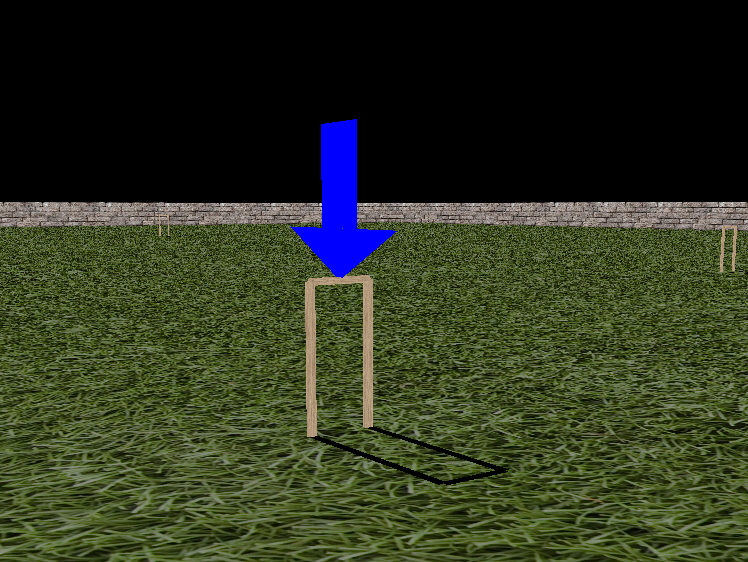
\includegraphics[width=4in]{goal.png}

Le premier joueur qui traverse les six cerceaux dans le bon ordre gagne.

\section*{Équations}

\subsection*{Méthodes numériques}

Nous avons encore une fois utilisé la méthode de Runge-Kutta d'ordre 4
afin de facilement résoudre nos équations différentielles. Ceci fut un
mauvais choix à cause d'une instabilité perçu dans certain cas
rare. De plus, étant donné que la force du au frottement de roulement
est constante, la méthode de Runge-Kutta n'a pas été beaucoup plus
précise que la méthode d'Euler.

\subsection*{Collisions}

Nous avons du gérer plusieurs collisions différentes mais elles
peuvent se regrouper en deux catégories. La première catégorie est
lorsqu'une balle entre en collision avec un objet qui ne bouge pas. La
deuxième catégorie est lorsque la balle entre en collision avec une
autre balle.

Nous avons traiter le maillet, les cerceaux, les murs et le poteau
comme des objets qui ne bougent pas. Ceci veut dire que lorsqu'une
balle entre en collision avec ces objets, seulement la vitesse et la
position de la balle sont modifiés.

Nous avons donc fait une réflection de la vitesse sur la normale de
collision multiplié par la coefficient de restitution afin de trouver
la vitesse de la balle après une collision.

Pour le cas d'une collision balle balle, nous avons utilisé des
équations de collisions inélastiques de sorte que:

\begin{flalign*}
  \epsilon_c = \frac{v_2 - v_1}{u_1 - u_2}
\end{flalign*}

$v_1$ est la vitesse scalaire de la première balle après l'impacte.

$v_2$ est la vitesse scalaire de la deuxième balle après l'impacte.

$u_1$ est la vitesse scalaire de la première balle avant l'impacte.

$u_2$ est la vitesse scalaire de la deuxième balle avant l'impacte.

\subsection*{Ombres}

Afin de créer l'illusion des ombres. Nous avons opté pour une solution
très simple. Nous avons créé une matrice de projection tel que la
matrice de projection orthonormale d'OpenGL. Nous avons appliqué cette
matrice à tous nos vertex d'un deuxième rendu de la scène. Ceci à fait
en sorte que tout les points de notre rendu se retrouvent sur notre
plan de gazon. Ce rendu étant noir nous donne l'effet d'ombres.

La matrice qui fait la projection orthogonale de vertex sur le plan
$xy$ avec un vecteur unitaire de direction $\vec{d}$ est:

\[ \left(
\begin{array}{cccc}
  1 & 0 & \frac{d_x}{d_z} & 0 \\
  0 & 1 & \frac{d_y}{d_z} & 0 \\
  0 & 0 & 0 & offset \\
  0 & 0 & 0 & 1
\end{array}
\right)\]

Le offset est supposé être nulle mais nous ne mettons pas une valeur
nulle car sinon le gazon et les ombres se battent dans le \begin{it}
  depth buffer \end{it} de OpenGL. Nous mettons donc une valeur qui
approche zéro tel que 0.001. De plus, dans notre programme, nous
entrons plutôt la transposé de cette matrice car OpenGL postmultiplie
ses matrices par la notre.

Nous avons opté pour cette approche plutôt que la méthode présenté car
nous avons eu des problèmes avec la compilation de fonctionnalités plus
avancé d'OpenGL en C++11.

\subsection*{Son}

Pour créer du son, nous avons utilisé des ondes sinusoïdales entre les
fréquence de 293 Hz et 1174 Hz. Afin de déterminer l'amplitude du son,
nous avons utilisé l'équation fournie dans l'énoncer:

\begin{flalign*}
  I = 100(1 + ln (\frac{v_r^2}{4} - 2 * (distance - 1)))
\end{flalign*}

Nous avons remarqué que les parenthèses n'étaient pas balancées dans
l'énoncer. Nous avons choisis cette interprétation car nous avons un
résultat de 100 db pour une distance de 1 met une vitesse relative de
2 m/s. De plus, avec cette équations, nous avions des résultats
vraisemblables; avec l'autre équation, nous avions des valeurs
négatives. Dans ce cas si par contre, nous pouvons avec des valeurs
négatives sous le ln.

\section*{Résultats}

Lors d'une collision avec le mur gauche.

\subsection*{Balle Mur}

\begin{verbatim}
Collision de la balle au point (-6.962000, -7.000000, 0.038000)
Vitesse initiale de (-3.681314, 0.000000, 0.000000).
Vitesse finale de (1.840657, 1.840657, 0.000000).
\end{verbatim}

Nous voyons que les résultats sont ceux auxquels nous sommes attendus
qui respectent nos contraintes établies lors de la section équations.

\subsection*{Balle Cerceau}

Lors d'une collision avec le cerceau 1.

\begin{verbatim}
Collision de la balle au point (-2.552619, -5.295424, 0.038000)
Vitesse initiale de (0.656115, 2.513160, 0.000000).
Vitesse finale de (0.290326, 0.290326, 0.000000).
\end{verbatim}

Encore une fois, ces résultats respectent les contraintes établies
précédemment.

\subsection*{Balle Balle}

\begin{verbatim}
Collision balle balle :
	Jaune
		pos = (-5.087142, -5.241385, 0.038000)
		vel initiale = (-1.030496, 1.666984, 0.000000)
		vel finale = (-0.576498, -0.016812, 0.000000)
	Bleu
		pos = (-5.102014, -5.180848, 0.038000)
		vel initiale = (0.000000, 0.000000, 0.000000)
		vel finale = (-0.453999, 1.683795, 0.000000)
\end{verbatim}

Ceci nous démontre que notre modèle de collisions inélastique est
suffisant.

\section*{Conclusion}

Nous avons eu plusieurs problèmes lors de ce projet. Un des problèmes
les plus important fut l'utilisation de la méthode de Runge-Kutta
4. Dans certains cas, lorsque les balles avaient des vitesses très
faibles, la méthode devenait instable. Lorsque ceci se produisait, la
vitesse oscillait et ne se stabilisait jamais ce qui faisait en sorte
qu'un tour ne finissait pas. Pour régler ceci, nous détectons quand la
méthode se met à osciller et nous annulons la vitesse (qui est déjà
très faible). Ceci n'est pas une solution idéale. Une meilleur
solution aurait été d'utiliser la méthode d'Euler implicite. Cette
méthode nous aurait garantie une certaine stabilité.

Un autre problème important fut le choix de l'utilisation du c++11. Le
problème ne vient pas du choix du c++ mais plutôt de la version 2011
qui vient tout juste de sortir. Étant donné sa nouveauté, peut de
compilateur la supporte partiellement. Étant donné que nous travaillons
sous Linux, nous avons eu de la misère à trouver un compilateur sous
Windows capable de supporter cette nouvelle version du c++. Nous
compilons donc sous Linux la version Linux et Windows. Le choix du
c++ nous a par contre permis d'avoir une application temps réelle avec
un taux de rafraîchissement tolérable.

L'incertitude de l'équation du son nous à causé problème car nous
avons longtemps utilisé la mauvaise interprétation de l'équation qui
nous retournait des db négatif et de l'ordre des -1000.

Un autre problème rencontré fut le fait que lors d'une collision, les
objets sont imbriqués l'un dans les autres. Pour réglé ceci, lorsque
nous détectons un objets qui est rentré dans un autre, on le déplace.

Certains bugs n'ont pas pu être réparé à temps pour le livrable. Le
bug le plus notable est lorsque le maillet frappe la balle très
légèrement, le jeu se retrouve parfois entre deux états. Ceci dure
indéfiniment et le jeux dois être redémarré.

Nous somme par contre très contents d'avoir choisi de faire
l'application en c++ et en temps réel car ceci nous a permit de
rencontrer plusieurs difficultés qui se sont présenté que nous
n'avions pas eu a s'occuper lors des travaux précédents.

Il serait intéressant d'essayer de faire ce jeu de croquet à partir
de tracer de rayons sur la carte graphique en temps réelle. Ceci
serait intéressant car nous pourrions appliquer les notions
d'optiques vu en cours en trois dimensions. De plus, un jeux de
croquet se porte bien au lancer de rayons car il est composé
principalement de formes que l'on peut facilement d'écrire à l'aide
d'équations.

\end{document}
